\section{Heat of Vaporization of Nitrogen}

\instructornote{%
Rewritten by Matt Trawick, 2015.  Time: pretty long (over 1 hour, if I recall?)

This lab requires students to understand electrical power, $P=IV$.  This pretty much demands that this lab (and probably all of thermodynamics, therefore) be done \textit{after} electric circuits.

Additional notes by Matt:

This version of this lab is based on an earlier version that gave a very prescriptive set of instructions for students.  (IMHO, it wasn't quite like filling out a tax form, with ``subtract line 13 from line 12,'' but it was close.)

In one of my 132 classes, when I had used the previous (more cook-booky)
version of this lab, I put a problem on an exam where I just gave students
a graph of weight \textit{vs.}~time for liquid nitrogen (part with heater on, part
with heater off, each with a different slope) and told them the current and
voltage of the heater, and  asked them to calculate the heat of vaporization.

Exactly 3 students out of 24 could do it.

So the next year I wrote this version of this lab, with many fewer
directions, basically making them figure out for themselves what to
do (presumably with some help from me when they got unstuck).  I put
the same question on a different exam and 16 out of 20 students could
do it (scoring 9 out of 10 points on the problem or above.) Based on
that data, I conclude that this more minimimalist version of this
lab is more effective.

When I have run this lab recently, \textit{a few} students just haven't gotten very good data.  For those students, I posted my own data online, telling them, ``okay, analyze this instead.''  That file, \filename{nitrogen\_trawick\_raw.xlsx}, is available on the Github repository.  I also posted there a file with some of my analysis, \filename{nitrogen\_trawick\_analysis.xlsx}, for other instructors. 

Some other experimental conclusions I drew:

\begin{itemize}[nosep]
\item The background boil-off rate varies by about a factor of two depending on how full the cup is.  I suspect that this is the biggest source of discrepancy for the students: they measure with power on when the cup is full, then measure with power off when the cup is half empty.  (This is especially a big deal if they choose a low heater power.)  So apparently it's important to refill the cups to the same level before each run.

\item I was curious whether I would see discrepancies at very high heater power due to gas given off at $T > 77$~K.  I saw no evidence of that, as I obtained quite reasonable numbers even with $V=30$ volts.

\item There's (possibly) a small effect of gas at $T>77$~K when the resistor is too close to the liquid surface.  (I was able to get a value for L about 7\% too high in that case.)  Be sure the resistor is down near the bottom of the cup.

\item For heater voltages of 20~V, 25~V, and 30~V, I got values of latent heat within 1\% of the accepted value.  For lower voltages my values are off by more like 5\% in either direction, suggesting I haven't adequately accounted for uncertainty in the slope measurement.
\end{itemize}
}

\makelabheader %(Space for student name, etc., defined in master.tex)

\bigskip

\begin{wrapfigure}[5]{r}{0.51\textwidth}
    \vspace{0.1in}
    \includegraphics[width=0.51\textwidth]{latent_heat_of_vaporization_of_nitrogen/heat_vap_nit_fig_1.eps}
\end{wrapfigure}

\bigskip

\textbf{Apparatus}
\begin{itemize}
\item Lab stand
\item Styrofoam cup
\item Liquid nitrogen
\item Power resistor
\item Power supply
\item Digital multimeter
  % 5/18/2015: Added the DMM back in.  Although the DMM is not strictly necessary (since our power supplies have current and voltage measurement on them) students should have a DMM in case they want to measure resistance or trouble-shoot something.
\item Wires
\item Pasco 550 interface
\item Force probe (with calibration weights)
\item \textit{Capstone} software (\filename{Liquid\_Nitrogen\_Vapor.cap} experiment file)
\end{itemize}
%\vspace{0.3cm}
%{\raggedleft \resizebox*{0.5\textwidth}{!}{\includegraphics{heat_vap_nit_fig_1.eps}} \par}
%\usepackage{wrapfig}
%\resizebox*{0.5\textwidth}{!}{\includegraphics{heat_vap_nit_fig_1.eps}} \par}
%\vspace{0.3cm}

Your task is to measure the latent heat of vaporization for nitrogen with the equipment given.
Your basic strategy will be to use a resistor ``heater'' to put a known amount of thermal
energy into a container of liquid nitrogen, and to simultaneously use a force probe to
measure the amount of nitrogen changed from a liquid into a gas.

Some points to keep in mind:

\begin{enumerate}

\item You can measure three quantities that can help you find the power
dissipated in the resistor: $I$, $V$, and $R$. Be aware that the ``$\!R$'' may change drastically with temperature.

\item Some liquid nitrogen will boil away even with your heater turned off, just due to lousy thermal insulation. You'll have to account for this somehow.

\item Check your force measurements with known weights to make sure your force probe is properly calibrated and not giving completely bogus results.  (To calibrate your force probe, see Appendix \ref{capstone}.) 

\item You will probably have to assume that the nitrogen gas given off is at exactly the same temperature as the liquid, even though it could be slightly hotter. Can you think of some good ways to either minimize this problem or account for it somehow?

\item Yes, you will need to estimate your uncertainty for this experiment. Does the accepted value for the latent heat of nitrogen fall within the range of your uncertainty?

\end{enumerate}

Good Luck!  :-)
